\section{单纯形法}
\subsection{单纯形法}
\begin{note}
    最优解一定在极点达到,而极点对应于基本可行解,求解线性规划问题归结为找最优基本可行解。\textbf{可以从一个基本可行解出发,求一个使目标函数值有所改善的基本可行解}:通过最优性条件判断是否达到最优解,并不断改进基本可行解,力图达到最优基本可行解。
\end{note}

\begin{note}
    对于线性规划问题
    \[
        (LP)\begin{cases}
            \min & f(x)=cx \\
            \subject & Ax=b \\
            & x \ge 0
        \end{cases}
    \]
    其中 $A$ 是 $m \times n$ 矩阵,秩为 $m$,$c$ 是 $n$ 维列向量,$b\ge 0$ 是 $m$ 维列向量.
    \begin{itemize}
        \item 初始基本可行解
            $A = (P_1, \dots, P_m, P_{m + 1}, \dots, P_n) = \begin{pmatrix}
                B & N
            \end{pmatrix}$

            基本解 $x^{(0)} = \begin{pmatrix}
                B^{-1}b \\
                0
            \end{pmatrix}$,若 $B^{-1}b \ge 0$,则 $x^{(0)}$ 是基本可行解.

            目标函数 $f_0 = cx^{(0)} = \begin{pmatrix}
                C_B & C_N
            \end{pmatrix} \begin{pmatrix}
                B^{-1}b \\
                0
            \end{pmatrix} = C_BB^{-1}b$
        \item 从初始基本可行解出发,求一个改进的基本可行解.
        \item 进基和终止条件
            \[
                x=\begin{pmatrix}
                    x_{B} \\
                    x_{N}
                \end{pmatrix}, Ax=b \Rightarrow\begin{pmatrix}
                    B & N
                \end{pmatrix}\begin{pmatrix}
                    x_{B} \\
                    x_{N}
                \end{pmatrix}=B x_{B}+N x_{N}=b \Rightarrow x_{B}=B^{-1}b-B^{-1} Nx_{N}
            \]
            目标函数值:
            \begin{align*}
                f = cx &= \begin{pmatrix}
                    c_B & c_N
                \end{pmatrix}\begin{pmatrix}
                    x_B \\
                    x_N
                \end{pmatrix} = c_Bx_B + c_Nx_N \\
                &= c_B(B^{-1}b - B^{-1}Nx_N) + c_Nx_N \\
                &= c_BB^{-1}b - (c_BB^{-1}N - c_N)x_N \\
                &= f_0 - \sum_{j\in R}(c_BB^{-1}P_j - c_j)x_j \quad R :\text{非基变量下标集} \\
                &=f_0 - \sum_{j\in R}(z_j - c_j)x_j
            \end{align*}
            \begin{enumerate}
                \item $z_j - c_j$ 称为检验数或判别数,基变量的检验数为0。
                \item 如果 $\forall j\in R$,有 $z_j - c_j \le 0$,则 $x^{(0)}$ 为最优解;
                \item 否则 $z_k - c_k = \underset{j \in R}{\max}\left\{z_j - c_j\right\}$,$P_k$ 为进基向量,$x_k$ 为进基变量,$x_k = 0 \to x_k > 0$.
            \end{enumerate}
        \item 出基下标和进基变量的值
        
            $Ax = b$ 解的变化,原 $x_B = B^{-1}b - B^{-1}Nx_N$,$x_k$ 由 0 变为正以后,$x_B = B^{-1}b - B^{-1}P_kx_k$,$x_B = \bar{b}-y_{k} x_{k}$,其中 $\bar{b} = B^{-1}b,y_k = B^{-1}P_k$.
            \begin{enumerate}
                \item 若 $y_{ik}\le 0$,则 $\forall x_k \Longrightarrow x_{B_i} > 0,x_k$ 可以取无限大,故 $f\to -\infty$,原问题无界.
                \item 要满足 $x_B = \bar{b}-y_{k} x_{k} \ge 0$,则取 $x_k = \min(\frac{\bar{b}}{y_{ik}},y_{ik}>0) = \frac{\bar{b}}{y_{rk}} > 0$,$r$ 为出基下标.
            \end{enumerate}
    \end{itemize}
\end{note}

\begin{note}
    单纯形法计算步骤
    \begin{enumerate}
        \item 初始基为 $B$,初始基本可行解为 $x^{(0)} = (B^{-1}b, 0)^t$,$\bar{b} = B^{-1}b$;
        \item 判断是否所有的 $c_BB^{-1}P_j - c_j \le 0$,即检验数是否全部非正,如果是,那么 $x^{(0)}$ 就是最优解,结束流程;
        \item 否则取 $z_k - c_k = \max\{z_j - c_j\} > 0$,判断是否 $y_k = B^{-1}P_k \le 0$,如果是,则解无界;
        \item 否则取 $\frac{\bar{b_r}}{y_{rk}} = \min\{\frac{\bar{b}_i}{y_{ik}} \mid y_{ik} > 0\}$,以 $p_k$ 代替 $P_{b_r}$ 换基,即 $x_{b_r}$ 为离基变量,$x_k$ 为进基变量,跳转步骤2。
    \end{enumerate}
\end{note}

\begin{note}
    单纯形表
    \begin{itemize}
        \item 做初等行变换
        \item 若 $z_j - c_j > 0$,对应的系数列向量 $\le 0$,则该 LP 存在无界解;
        \item 若某个非基变量的检验数为 0,则该 LP 存在多个最优解.
    \end{itemize}
    \begin{figure}[htbp]
        \centering
        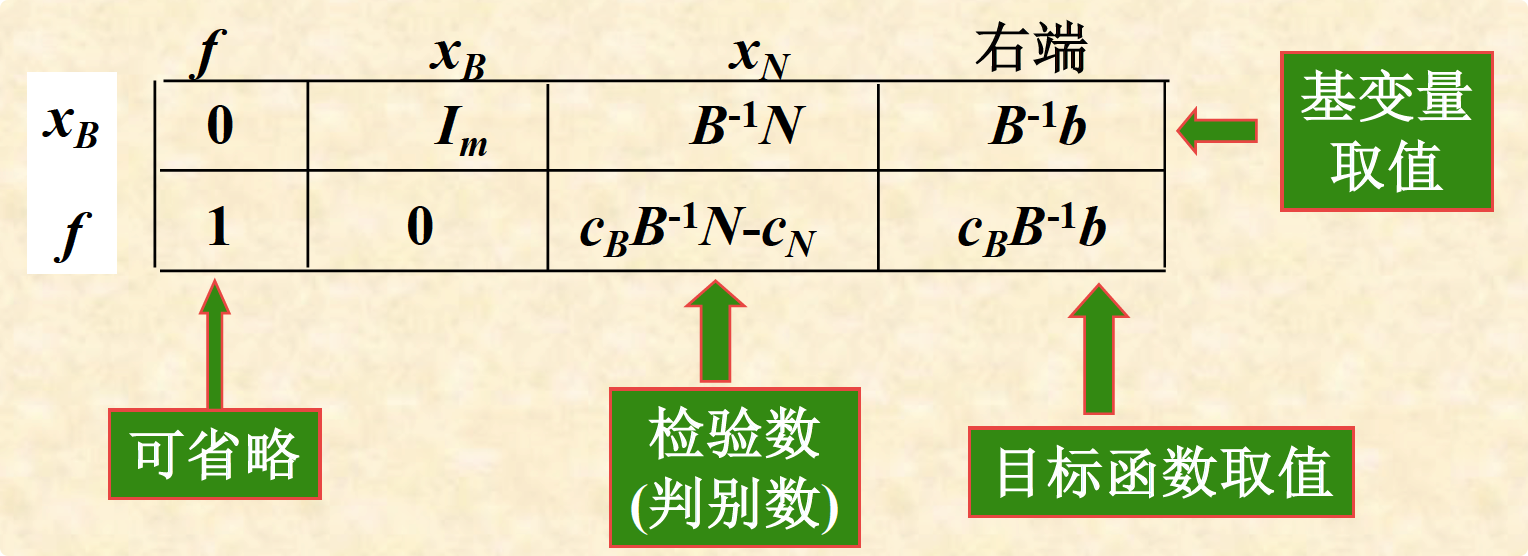
\includegraphics[width=0.8\textwidth]{./figures/img1.png}
        \caption{单纯形表 \label{fig1}}
    \end{figure}
\end{note}

\begin{example}
    用单纯形法求最优解
    \[
        \begin{cases}
            \min \quad &-x_2 + 2x_3\\
            \subject \quad &x_1 - 2x_2 + x_3 = 2\\
            &x_2 - 3x_3 \le 1\\
            x_2 - x_3 \le 2\\
            x_1, x_2, x_3 \ge 0
        \end{cases}  
    \]

    \answer 引入松弛变量化为标准形
    \[
        \begin{cases}
            \min \quad &-x_2 + 2x_3\\
            \subject \quad &x_1 - 2x_2 + x_3 = 2\\
            &x_2 - 3x_3 + x_4 = 1\\
            &x_2 - x_3 + x_5 = 2\\
            &x_1, x_2, x_3, x_4, x_5 \ge 0
        \end{cases}    
    \]
    选择初始基 $B = (P_1, P_4, P_5) = I$。
    \begin{center}
        \begin{tabular}{c|ccccc|c}
            & $x_1$ & $x_2$ & $x_3$ & $x_4$ & $x_5$ & \\
            \hline
            $x_1$ & 1 & -2 & 1 & 0 & 0 & 2\\
            $x_4$ & 0 & {\color{red} 1} & -3 & 1 & 0 & 1\\
            $x_5$ & 0 & 1 & -1 & 0 & 1 & 2\\
            \hline
             & 0 & 1 & -2 & 0 & 0 & 0
        \end{tabular}

        选取检验数最大的列,最大的列中 $\frac{1}{1} < \frac{2}{1}$

        \begin{tabular}{c|ccccc|c}
            & $x_1$ & $x_2$ & $x_3$ & $x_4$ & $x_5$ & \\
            \hline
            $x_1$ & 1 & 0 & -5 & 2 & 0 & 4\\
            $x_2$ & 0 & 1 & -3 & 1 & 0 & 1\\
            $x_5$ & 0 & 0 & {\color{red} 2} & -1 & 1 & 1\\
            \hline
            & 0 & 0 & 1 & -1 & 0 & -1
        \end{tabular}
        
        选取检验数最大的列,最大的列中只有 $\frac{1}{2}$可选

        \begin{tabular}{c|ccccc|c}
            & $x_1$ & $x_2$ & $x_3$ & $x_4$ & $x_5$ & \\
            \hline
            $x_1$ & 1 & 0 & 0 & -1/2 & 5/2 & 13/2\\
            $x_2$ & 0 & 1 & 0 & -1/2 & 3/2 & 5/2\\
            $x_3$ & 0 & 0 & 1 & -1/2 & 1/2 & 1/2\\
            \hline
             & 0 & 0 & 0 & -1/2 & -1/2 & -3/2
        \end{tabular}
    \end{center}
    可得 $x^* = \left(\frac{13}{2}, \frac{5}{2}, \frac{1}{2}\right)^t$,$f_{\min} = -\frac{3}{2}$。
\end{example}

\begin{example}
    用单纯形法求最优解
    \[
        \begin{cases}
            \max \quad &2x_1 + x_2 - x_3\\
            \subject \quad &x_1 + x_2 + 2x_3 \le 6\\
            &x_1 + 4x_2 - x_3 \le 4\\
            &x_1, x_2, x_3 \ge 0
        \end{cases}    
    \]
    引入松弛变量化为标准形
    \[
        \begin{cases}
            \max \quad &2x_1 + x_2 - x_3\\
            \subject \quad &x_1 + x_2 + 2x_3 + x_4 = 6\\
            &x_1 + 4x_2 - x_3 + x_5 = 4\\
            &x_1, x_2, x_3, x_4, x_5 \ge 0
        \end{cases}    
    \]
    选择初始基 $B = (P_4, P_5) = I$。
    \begin{center}
        \begin{tabular}{c|ccccc|c}
            & $x_1$ & $x_2$ & $x_3$ & $x_4$ & $x_5$ & \\
            \hline
            $x_4$ & 1 & 1 & 2 &1 & 0 & 6\\
            $x_5$ & {\color{red} 1} & 4 & -1 & 0 & 1 & 4\\
            \hline
             & -2 & -1 & 1 & 0 & 0 & 0
        \end{tabular}

        选取检验数最小的列,其中 $\frac{4}{1} < \frac{6}{1}$

        \begin{tabular}{c|ccccc|c}
            & $x_1$ & $x_2$ & $x_3$ & $x_4$ & $x_5$ & \\
            \hline
            $x_4$ & 0 & -3 & {\color{red}3} & 1 & -1 & 2\\
            $x_1$ & 1 & 4 & -1 & 0 & 1 & 4\\
            \hline
             & 0 & 7 & -1 & 0 & 2 & 8
        \end{tabular}

        选取检验数最小的列,只有 $\frac{3}{2}$

        \begin{tabular}{c|ccccc|c}
            & $x_1$ & $x_2$ & $x_3$ & $x_4$ & $x_5$ & \\
            \hline
            $x_4$ & 0 & -1 & 1 & 1/3 & -1/3 & 2/3\\
            $x_1$ & 1 & 3 & 0 & 1/3 & 2/3 & 14/3\\
            \hline
             & 0 & 6 & 0 & 1/3 & 5/3 & 26/3
        \end{tabular}
    \end{center}
    故 $x^* = \left(\frac{14}{3}, 0, \frac{2}{3}\right)^t$,$f_{\max} = \frac{26}{3}$。
\end{example}

\subsection{两阶段法}
(感觉很useless啊)

对于如下线性规划问题
\[
    \begin{cases}
        \min \quad &c^tx\\
        \subject \quad &Ax = b\\
        &x \ge 0
    \end{cases}    
\]
两阶段法步骤:
\begin{enumerate}
    \item 用单纯形法把人工变量变为非基变量,求出原问题的一个基本可行解。

    求解下列模型
    \[
        \begin{cases}
            \min \quad &e^tx_a\\
            \subject \quad &Ax + x_a = b\\
            &e = (1, \dots, 1)^t\\
            &x, x_a \ge 0
        \end{cases}
    \]
    得到最优解为 $(\bar{x}^t, \bar{x}_a^t)^t$,最优值为 $e^t\bar{x}_a$。
    \begin{enumerate}
        \item 若 $\bar{x}^a \neq 0$,则无可行解
        \item $\bar{x}_a = 0$ 而且所有的人工变量都是非基变量,则 $\bar{x}$ 是基本可行解
        \item $\bar{x}_a = 0$ 但 $\bar{x}_a$ 的某个分量 $\bar{x}_{a_j}$ 为基变量,则设法将 $\bar{x}_{a_j}$ 从基变量中去掉。
    \end{enumerate}
    \item 从得到的基本可行解出发,用单纯形法求最优解。
\end{enumerate}

\subsection{线性规划的最优性条件}
即KKT条件。

对于如下凸优化问题
\[
    \begin{cases}
        \min \quad &f(x)\\
        \subject \quad &f_i(x) \le 0, 1 \le i \le m\\
        &h_i(x) = 0, 1 \le i \le p
    \end{cases}    
\]
有拉格朗日函数 $L(x, \lambda, \mu) = f(x) + \sum \lambda_if_i(x) + \sum \mu_ih_i(x)$.

$x$ 是最优解当且仅当
\begin{enumerate}
    \item 满足约束条件:$f_i(x) \le 0$,$h_i(x) = 0$
    \item 非负约束:$\lambda \succeq 0$
    \item 互补松弛:$\lambda_if_i(x) = 0$
    \item $\partial_xL(x, \lambda, \mu) = 0$
\end{enumerate}